
%% bare_jrnl.tex
%% V1.3
%% 2007/01/11
%% by Michael Shell
%% see http://www.michaelshell.org/
%% for current contact information.
%%
%% This is a skeleton file demonstrating the use of IEEEtran.cls
%% (requires IEEEtran.cls version 1.7 or later) with an IEEE journal paper.
%%
%% Support sites:
%% http://www.michaelshell.org/tex/ieeetran/
%% http://www.ctan.org/tex-archive/macros/latex/contrib/IEEEtran/
%% and
%% http://www.ieee.org/



% *** Authors should verify (and, if needed, correct) their LaTeX system  ***
% *** with the testflow diagnostic prior to trusting their LaTeX platform ***
% *** with production work. IEEE's font choices can trigger bugs that do  ***
% *** not appear when using other class files.                            ***
% The testflow support page is at:
% http://www.michaelshell.org/tex/testflow/


%%*************************************************************************
%% Legal Notice:
%% This code is offered as-is without any warranty either expressed or
%% implied; without even the implied warranty of MERCHANTABILITY or
%% FITNESS FOR A PARTICULAR PURPOSE! 
%% User assumes all risk.
%% In no event shall IEEE or any contributor to this code be liable for
%% any damages or losses, including, but not limited to, incidental,
%% consequential, or any other damages, resulting from the use or misuse
%% of any information contained here.
%%
%% All comments are the opinions of their respective authors and are not
%% necessarily endorsed by the IEEE.
%%
%% This work is distributed under the LaTeX Project Public License (LPPL)
%% ( http://www.latex-project.org/ ) version 1.3, and may be freely used,
%% distributed and modified. A copy of the LPPL, version 1.3, is included
%% in the base LaTeX documentation of all distributions of LaTeX released
%% 2003/12/01 or later.
%% Retain all contribution notices and credits.
%% ** Modified files should be clearly indicated as such, including  **
%% ** renaming them and changing author support contact information. **
%%
%% File list of work: IEEEtran.cls, IEEEtran_HOWTO.pdf, bare_adv.tex,
%%                    bare_conf.tex, bare_jrnl.tex, bare_jrnl_compsoc.tex
%%*************************************************************************

% Note that the a4paper option is mainly intended so that authors in
% countries using A4 can easily print to A4 and see how their papers will
% look in print - the typesetting of the document will not typically be
% affected with changes in paper size (but the bottom and side margins will).
% Use the testflow package mentioned above to verify correct handling of
% both paper sizes by the user's LaTeX system.
%
% Also note that the "draftcls" or "draftclsnofoot", not "draft", option
% should be used if it is desired that the figures are to be displayed in
% draft mode.
%
\documentclass[journal,twoside]{IEEEtran}
\usepackage{blindtext}
\usepackage{graphicx}
\usepackage{textcomp}
\usepackage{subfig}
\usepackage{multirow}
\usepackage{authblk}

% Some very useful LaTeX packages include:
% (uncomment the ones you want to load)


% *** MISC UTILITY PACKAGES ***
%
%\usepackage{ifpdf}
% Heiko Oberdiek's ifpdf.sty is very useful if you need conditional
% compilation based on whether the output is pdf or dvi.
% usage:
% \ifpdf
%   % pdf code
% \else
%   % dvi code
% \fi
% The latest version of ifpdf.sty can be obtained from:
% http://www.ctan.org/tex-archive/macros/latex/contrib/oberdiek/
% Also, note that IEEEtran.cls V1.7 and later provides a builtin
% \ifCLASSINFOpdf conditional that works the same way.
% When switching from latex to pdflatex and vice-versa, the compiler may
% have to be run twice to clear warning/error messages.






% *** CITATION PACKAGES ***
%
%\usepackage{cite}
% cite.sty was written by Donald Arseneau
% V1.6 and later of IEEEtran pre-defines the format of the cite.sty package
% \cite{} output to follow that of IEEE. Loading the cite package will
% result in citation numbers being automatically sorted and properly
% "compressed/ranged". e.g., [1], [9], [2], [7], [5], [6] without using
% cite.sty will become [1], [2], [5]--[7], [9] using cite.sty. cite.sty's
% \cite will automatically add leading space, if needed. Use cite.sty's
% noadjust option (cite.sty V3.8 and later) if you want to turn this off.
% cite.sty is already installed on most LaTeX systems. Be sure and use
% version 4.0 (2003-05-27) and later if using hyperref.sty. cite.sty does
% not currently provide for hyperlinked citations.
% The latest version can be obtained at:
% http://www.ctan.org/tex-archive/macros/latex/contrib/cite/
% The documentation is contained in the cite.sty file itself.






% *** GRAPHICS RELATED PACKAGES ***
%
\ifCLASSINFOpdf
  % \usepackage[pdftex]{graphicx}
  % declare the path(s) where your graphic files are
  % \graphicspath{{../pdf/}{../jpeg/}}
  % and their extensions so you won't have to specify these with
  % every instance of \includegraphics
  % \DeclareGraphicsExtensions{.pdf,.jpeg,.png}
\else
  % or other class option (dvipsone, dvipdf, if not using dvips). graphicx
  % will default to the driver specified in the system graphics.cfg if no
  % driver is specified.
  % \usepackage[dvips]{graphicx}
  % declare the path(s) where your graphic files are
  % \graphicspath{{../eps/}}
  % and their extensions so you won't have to specify these with
  % every instance of \includegraphics
  % \DeclareGraphicsExtensions{.eps}
\fi
% graphicx was written by David Carlisle and Sebastian Rahtz. It is
% required if you want graphics, photos, etc. graphicx.sty is already
% installed on most LaTeX systems. The latest version and documentation can
% be obtained at: 
% http://www.ctan.org/tex-archive/macros/latex/required/graphics/
% Another good source of documentation is "Using Imported Graphics in
% LaTeX2e" by Keith Reckdahl which can be found as epslatex.ps or
% epslatex.pdf at: http://www.ctan.org/tex-archive/info/
%
% latex, and pdflatex in dvi mode, support graphics in encapsulated
% postscript (.eps) format. pdflatex in pdf mode supports graphics
% in .pdf, .jpeg, .png and .mps (metapost) formats. Users should ensure
% that all non-photo figures use a vector format (.eps, .pdf, .mps) and
% not a bitmapped formats (.jpeg, .png). IEEE frowns on bitmapped formats
% which can result in "jaggedy"/blurry rendering of lines and letters as
% well as large increases in file sizes.
%
% You can find documentation about the pdfTeX application at:
% http://www.tug.org/applications/pdftex





% *** MATH PACKAGES ***
%
%\usepackage[cmex10]{amsmath}
% A popular package from the American Mathematical Society that provides
% many useful and powerful commands for dealing with mathematics. If using
% it, be sure to load this package with the cmex10 option to ensure that
% only type 1 fonts will utilized at all point sizes. Without this option,
% it is possible that some math symbols, particularly those within
% footnotes, will be rendered in bitmap form which will result in a
% document that can not be IEEE Xplore compliant!
%
% Also, note that the amsmath package sets \interdisplaylinepenalty to 10000
% thus preventing page breaks from occurring within multiline equations. Use:
%\interdisplaylinepenalty=2500
% after loading amsmath to restore such page breaks as IEEEtran.cls normally
% does. amsmath.sty is already installed on most LaTeX systems. The latest
% version and documentation can be obtained at:
% http://www.ctan.org/tex-archive/macros/latex/required/amslatex/math/





% *** SPECIALIZED LIST PACKAGES ***
%
%\usepackage{algorithmic}
% algorithmic.sty was written by Peter Williams and Rogerio Brito.
% This package provides an algorithmic environment fo describing algorithms.
% You can use the algorithmic environment in-text or within a figure
% environment to provide for a floating algorithm. Do NOT use the algorithm
% floating environment provided by algorithm.sty (by the same authors) or
% algorithm2e.sty (by Christophe Fiorio) as IEEE does not use dedicated
% algorithm float types and packages that provide these will not provide
% correct IEEE style captions. The latest version and documentation of
% algorithmic.sty can be obtained at:
% http://www.ctan.org/tex-archive/macros/latex/contrib/algorithms/
% There is also a support site at:
% http://algorithms.berlios.de/index.html
% Also of interest may be the (relatively newer and more customizable)
% algorithmicx.sty package by Szasz Janos:
% http://www.ctan.org/tex-archive/macros/latex/contrib/algorithmicx/




% *** ALIGNMENT PACKAGES ***
%
%\usepackage{array}
% Frank Mittelbach's and David Carlisle's array.sty patches and improves
% the standard LaTeX2e array and tabular environments to provide better
% appearance and additional user controls. As the default LaTeX2e table
% generation code is lacking to the point of almost being broken with
% respect to the quality of the end results, all users are strongly
% advised to use an enhanced (at the very least that provided by array.sty)
% set of table tools. array.sty is already installed on most systems. The
% latest version and documentation can be obtained at:
% http://www.ctan.org/tex-archive/macros/latex/required/tools/


%\usepackage{mdwmath}
%\usepackage{mdwtab}
% Also highly recommended is Mark Wooding's extremely powerful MDW tools,
% especially mdwmath.sty and mdwtab.sty which are used to format equations
% and tables, respectively. The MDWtools set is already installed on most
% LaTeX systems. The lastest version and documentation is available at:
% http://www.ctan.org/tex-archive/macros/latex/contrib/mdwtools/


% IEEEtran contains the IEEEeqnarray family of commands that can be used to
% generate multiline equations as well as matrices, tables, etc., of high
% quality.


%\usepackage{eqparbox}
% Also of notable interest is Scott Pakin's eqparbox package for creating
% (automatically sized) equal width boxes - aka "natural width parboxes".
% Available at:
% http://www.ctan.org/tex-archive/macros/latex/contrib/eqparbox/





% *** SUBFIGURE PACKAGES ***
%\usepackage[tight,footnotesize]{subfigure}
% subfigure.sty was written by Steven Douglas Cochran. This package makes it
% easy to put subfigures in your figures. e.g., "Figure 1a and 1b". For IEEE
% work, it is a good idea to load it with the tight package option to reduce
% the amount of white space around the subfigures. subfigure.sty is already
% installed on most LaTeX systems. The latest version and documentation can
% be obtained at:
% http://www.ctan.org/tex-archive/obsolete/macros/latex/contrib/subfigure/
% subfigure.sty has been superceeded by subfig.sty.



%\usepackage[caption=false]{caption}
%\usepackage[font=footnotesize]{subfig}
% subfig.sty, also written by Steven Douglas Cochran, is the modern
% replacement for subfigure.sty. However, subfig.sty requires and
% automatically loads Axel Sommerfeldt's caption.sty which will override
% IEEEtran.cls handling of captions and this will result in nonIEEE style
% figure/table captions. To prevent this problem, be sure and preload
% caption.sty with its "caption=false" package option. This is will preserve
% IEEEtran.cls handing of captions. Version 1.3 (2005/06/28) and later 
% (recommended due to many improvements over 1.2) of subfig.sty supports
% the caption=false option directly:
%\usepackage[caption=false,font=footnotesize]{subfig}
%
% The latest version and documentation can be obtained at:
% http://www.ctan.org/tex-archive/macros/latex/contrib/subfig/
% The latest version and documentation of caption.sty can be obtained at:
% http://www.ctan.org/tex-archive/macros/latex/contrib/caption/




% *** FLOAT PACKAGES ***
%
%\usepackage{fixltx2e}
% fixltx2e, the successor to the earlier fix2col.sty, was written by
% Frank Mittelbach and David Carlisle. This package corrects a few problems
% in the LaTeX2e kernel, the most notable of which is that in current
% LaTeX2e releases, the ordering of single and double column floats is not
% guaranteed to be preserved. Thus, an unpatched LaTeX2e can allow a
% single column figure to be placed prior to an earlier double column
% figure. The latest version and documentation can be found at:
% http://www.ctan.org/tex-archive/macros/latex/base/



%\usepackage{stfloats}
% stfloats.sty was written by Sigitas Tolusis. This package gives LaTeX2e
% the ability to do double column floats at the bottom of the page as well
% as the top. (e.g., "\begin{figure*}[!b]" is not normally possible in
% LaTeX2e). It also provides a command:
%\fnbelowfloat
% to enable the placement of footnotes below bottom floats (the standard
% LaTeX2e kernel puts them above bottom floats). This is an invasive package
% which rewrites many portions of the LaTeX2e float routines. It may not work
% with other packages that modify the LaTeX2e float routines. The latest
% version and documentation can be obtained at:
% http://www.ctan.org/tex-archive/macros/latex/contrib/sttools/
% Documentation is contained in the stfloats.sty comments as well as in the
% presfull.pdf file. Do not use the stfloats baselinefloat ability as IEEE
% does not allow \baselineskip to stretch. Authors submitting work to the
% IEEE should note that IEEE rarely uses double column equations and
% that authors should try to avoid such use. Do not be tempted to use the
% cuted.sty or midfloat.sty packages (also by Sigitas Tolusis) as IEEE does
% not format its papers in such ways.


%\ifCLASSOPTIONcaptionsoff
%  \usepackage[nomarkers]{endfloat}
% \let\MYoriglatexcaption\caption
% \renewcommand{\caption}[2][\relax]{\MYoriglatexcaption[#2]{#2}}
%\fi
% endfloat.sty was written by James Darrell McCauley and Jeff Goldberg.
% This package may be useful when used in conjunction with IEEEtran.cls'
% captionsoff option. Some IEEE journals/societies require that submissions
% have lists of figures/tables at the end of the paper and that
% figures/tables without any captions are placed on a page by themselves at
% the end of the document. If needed, the draftcls IEEEtran class option or
% \CLASSINPUTbaselinestretch interface can be used to increase the line
% spacing as well. Be sure and use the nomarkers option of endfloat to
% prevent endfloat from "marking" where the figures would have been placed
% in the text. The two hack lines of code above are a slight modification of
% that suggested by in the endfloat docs (section 8.3.1) to ensure that
% the full captions always appear in the list of figures/tables - even if
% the user used the short optional argument of \caption[]{}.
% IEEE papers do not typically make use of \caption[]'s optional argument,
% so this should not be an issue. A similar trick can be used to disable
% captions of packages such as subfig.sty that lack options to turn off
% the subcaptions:
% For subfig.sty:
% \let\MYorigsubfloat\subfloat
% \renewcommand{\subfloat}[2][\relax]{\MYorigsubfloat[]{#2}}
% For subfigure.sty:
% \let\MYorigsubfigure\subfigure
% \renewcommand{\subfigure}[2][\relax]{\MYorigsubfigure[]{#2}}
% However, the above trick will not work if both optional arguments of
% the \subfloat/subfig command are used. Furthermore, there needs to be a
% description of each subfigure *somewhere* and endfloat does not add
% subfigure captions to its list of figures. Thus, the best approach is to
% avoid the use of subfigure captions (many IEEE journals avoid them anyway)
% and instead reference/explain all the subfigures within the main caption.
% The latest version of endfloat.sty and its documentation can obtained at:
% http://www.ctan.org/tex-archive/macros/latex/contrib/endfloat/
%
% The IEEEtran \ifCLASSOPTIONcaptionsoff conditional can also be used
% later in the document, say, to conditionally put the References on a 
% page by themselves.





% *** PDF, URL AND HYPERLINK PACKAGES ***
%
%\usepackage{url}
% url.sty was written by Donald Arseneau. It provides better support for
% handling and breaking URLs. url.sty is already installed on most LaTeX
% systems. The latest version can be obtained at:
% http://www.ctan.org/tex-archive/macros/latex/contrib/misc/
% Read the url.sty source comments for usage information. Basically,
% \url{my_url_here}.





% *** Do not adjust lengths that control margins, column widths, etc. ***
% *** Do not use packages that alter fonts (such as pslatex).         ***
% There should be no need to do such things with IEEEtran.cls V1.6 and later.
% (Unless specifically asked to do so by the journal or conference you plan
% to submit to, of course. )


% correct bad hyphenation here
%\hyphenation{op-tical net-works semi-conduc-tor}


\begin{document}
\setcounter{page}{23}
%
% paper title
% can use linebreaks \\ within to get better formatting as desired
\title{Identifying Dementia in MRI Scans using Artificial Neural Network and K-Nearest Neighbor}
%
%
% author names and IEEE memberships
% note positions of commas and nonbreaking spaces ( ~ ) LaTeX will not break
% a structure at a ~ so this keeps an author's name from being broken across
% two lines.
% use \thanks{} to gain access to the first footnote area
% a separate \thanks must be used for each paragraph as LaTeX2e's \thanks
% was not built to handle multiple paragraphs
%

%\author{Abinash~Manandhar, Dharma~K.~Shrestha, Sagar~Gautam, Sujan~Sauden, Dibakar R. Pant
%\author[1]{Abinash Manandhar}
%\author[2]{Sagar Gautam} 
%\author[3]{Dharma K. Shrestha}
%\author[4]{Sujan Sauden} 
%\author[5]{Dibakar R. Pant (PhD)}
%\renewcommand\Authands{ and }

\author{\IEEEauthorblockN{Abinash Manandhar\IEEEauthorrefmark{1},
Sagar Gautam\IEEEauthorrefmark{2}, 
Dharma K. Shrestha\IEEEauthorrefmark{3},
Sujan Sauden\IEEEauthorrefmark{4} and
Dibakar R. Pant\IEEEauthorrefmark{5}}
\IEEEauthorblockA{ \\Department of Electronics and Computer Engineering\\
Central Campus, Institute of Engineering, Tribhuvan University\\
\IEEEauthorrefmark{1}abinash.mdr@gmail.com,
\IEEEauthorrefmark{2}sagautam5@gmail.com,
\IEEEauthorrefmark{3}sht.dharma@gmail.com,
\IEEEauthorrefmark{4}sauden.2013@gmail.com,
\IEEEauthorrefmark{5}pdibakar@gmail.com}}


%,~\IEEEmembership{Student,~IOE}
%\thanks{Abinash Manandhar, Dharma K. Shrestha, Sagar Gautam and Sujan Sauden are students under the Department of Electronics and Computer Engineering, Central Campus, Institute of Engineering, Tribhuvan University, Pulchowk, Lalitpur.}}% <-this % stops a space

% note the % following the last \IEEEmembership and also \thanks - 
% these prevent an unwanted space from occurring between the last author name
% and the end of the author line. i.e., if you had this:
% 
% \author{....lastname \thanks{...} \thanks{...} }
%                     ^------------^------------^----Do not want these spaces!
%
% a space would be appended to the last name and could cause every name on that
% line to be shifted left slightly. This is one of those "LaTeX things". For
% instance, "\textbf{A} \textbf{B}" will typeset as "A B" not "AB". To get
% "AB" then you have to do: "\textbf{A}\textbf{B}"
% \thanks is no different in this regard, so shield the last } of each \thanks
% that ends a line with a % and do not let a space in before the next \thanks.
% Spaces after \IEEEmembership other than the last one are OK (and needed) as
% you are supposed to have spaces between the names. For what it is worth,
% this is a minor point as most people would not even notice if the said evil
% space somehow managed to creep in.


\markboth{Zerone Scholar,~Vol.~1, No.~1, November~2016}%
{Manandhar \MakeLowercase{\textit{et al.}}: Identifying Dementia in MRI Scans}

% The paper headers
%\markboth{Journal of \LaTeX\ Class Files,~Vol.~6, No.~1, January~2007}%
%{Shell \MakeLowercase{\textit{et al.}}: Bare Demo of IEEEtran.cls for Journals}
% The only time the second header will appear is for the odd numbered pages
% after the title page when using the twoside option.
% 
% *** Note that you probably will NOT want to include the author's ***
% *** name in the headers of peer review papers.                   ***
% You can use \ifCLASSOPTIONpeerreview for conditional compilation here if
% you desire.




% If you want to put a publisher's ID mark on the page you can do it like
% this:
%\IEEEpubid{0000--0000/00\$00.00~\copyright~2007 IEEE}
% Remember, if you use this you must call \IEEEpubidadjcol in the second
% column for its text to clear the IEEEpubid mark.



% use for special paper notices
%\IEEEspecialpapernotice{(Invited Paper)}




% make the title area
\maketitle

\begin{abstract}
%\boldmath
Artificial Neural Network (ANN) and K-Nearest Neighbor (KNN) models are used to detect dementia in MRI scans. Each scan is segmented and then normalized into four discrete color areas corresponding to white matter, dark gray matter, light gray matter and black background, the former three constituting the feature set. Thresholding technique is used in segmentation and nearest neighbor interpolation technique is used in normalization of the images. The ANN implementation resulted into 69.81\% accuracy and the KNN implementation resulted into 81.13\% accuracy in classification of demented and non-demented scans.
\end{abstract}
% IEEEtran.cls defaults to using nonbold math in the Abstract.
% This preserves the distinction between vectors and scalars. However,
% if the journal you are submitting to favors bold math in the abstract,
% then you can use LaTeX's standard command \boldmath at the very start
% of the abstract to achieve this. Many IEEE journals frown on math
% in the abstract anyway.

% Note that keywords are not normally used for peerreview papers.
\begin{IEEEkeywords}
Dementia, MRI, ANN, KNN.
\end{IEEEkeywords}


% For peer review papers, you can put extra information on the cover
% page as needed:
% \ifCLASSOPTIONpeerreview
% \begin{center} \bfseries EDICS Category: 3-BBND \end{center}
% \fi
%
% For peerreview papers, this IEEEtran command inserts a page break and
% creates the second title. It will be ignored for other modes.
\IEEEpeerreviewmaketitle

\section{Introduction}
Dementia is a broad category of neuro-degenerative diseases, including, but not limited to, Alzheimer \textquotesingle s Disease, that causes a long term and often gradual decline in the patient\textquotesingle s ability to think and remember.[1] 
\par Dementia is a leading cause of deaths today; it affects more than 44 million people worldwide with every 1 out of 20 patients under the age of 65. The global cost of caring for dementia is estimated to be \$605 billion, which is equivalent to 1\% of the global gross domestic product.[1]
\par Diagnosis of dementia is conventionally done through cognitive, neurological and neuropsychological evaluation of a patient\textquotesingle s mental state. These tests, however, can not provide tangible measure of severity and proper indication of the suitable treatment.[2]
\par Neuroimaging in dementing illness has undergone revolutionary changes in recent years with the wide availability of an unprecedented array of new techniques. Machine Resonance Imaging (MRI), in particular, has aided in objective analysis for determining the presence and subsequently the type of dementia. Radiological findings may support the diagnosis of specific neurodegenerative disorders and sometimes radiological findings are necessary to confirm the diagnosis. It is a challenge for neuroimaging to contribute to the early diagnosis of neurodegenerative diseases such as Alzheimer\textquotesingle s disease. Early diagnosis includes recognition of pre-dementia conditions, such as mild cognitive impairment (MCI). [3]
\par Timely diagnosis of Dementia is vital in developing early treatments and designing management strategies to this fatal disease, but only 1 in every 4 people with Alzheimer\textquotesingle s or related dementia have been properly diagnosed.[1] This raises a need for easy and non-invasive technique for dementia diagnosis.
\par Previous researches in this field have used naive Bayesian classifier[4,5], C4.5 decision tree[4,6,8], support vector machine (SVM)[5,7], neural network[7] and multi-modality classification framework[9]. These have resulted in average accuracy of around 80\%. 
\par This project uses Artificial Neural Network and K-Nearest Neighbor approaches to classify MR Images into demented and non-demented categories.
\section{Data}
This project uses a dataset containing 436 neurological MRI scans made available by the Open Access Series of Imaging Studies (OASIS) project. This data set consists of a cross-sectional collection of 416 subjects covering the adult life span aged 18 to 96 including individuals with early to mild to moderate Alzheimer\textquotesingle s Disease. For each subject, 3 or 4 individual T1-weighted MRI scans obtained within a single imaging session are included. Each scan includes age, sex, education level, socioeconomic status, intracranial volume, and normalized brain volume, and two indicators of dementia: the clinical dementia rating (CDR) and minimental state exam (MMSE) associated with additional information about the subject. 
\begin{figure}[h!]
\centering
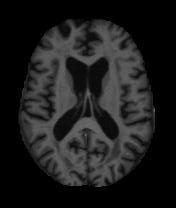
\includegraphics[width=2.05in]{5.jpg}
\DeclareGraphicsExtensions.
\caption{Original Image Slice}
\end{figure}
\par All images are in 16bit Bigendian Analyze 7.5 format. Each scan consists of 3D images of dimension 176x208x176 voxels which have been preprocessed to remove the skull, leaving only brain matter in the images.[10] 
\par The available data is divided into 12 discs with a total of 235 data sets containing enough information about dementia. Undemented MRI scans have Clinical Dementia Rating(CDR) value 0. Demented MRI scans have Clinical Dementia Rating(CDR) value of 0.5, 1, 1.5 or 2 depending on the severity of dementia.
\section{Methodology}
\subsection{Image Preprocessing}
Image files of the MRI scans from OASIS consists of raw information about each voxel. This image can not be used directly to model a image classification system since this image consists of large number of features and analysis of such features increases the complexity in modeling a classifier. So, image preprocessing should be performed in order to reduce some unnecessary features and preserve others that bear significance in dementia detection. Image preprocessing includes format conversion, image re-sampling, grayscale color enhancement, noise removal, segmentation, image normalization and finally feature extraction.\newline
\subsubsection{Segmentation}
Thresholding technique is used for segmentation of 3D images into four different volumes which are image background, white matter or the cerebro-spinal volume of the brain, the dark gray matter or the tissues inside the brain and the light gray matter (intermediate tissues between Gray matter and CSF).
\begin{figure}[h]
\centering
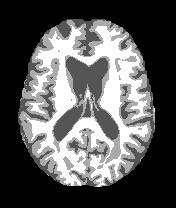
\includegraphics[width=2.05in]{9.jpg}
\DeclareGraphicsExtensions.
\caption{Segmented Image Slice}
\end{figure}
\newline The grayscale values and representative values of each of the volumes are:
\begin{table}[h]
\centering
\begin{tabular}{|c|c|c|}
	\hline
	Particulars & Grayscale Value & Representative Value\\
	\hline
	Background & 0-5 & 0\\
	Dark Gray Matter &  5-38 & 85\\
	Light Gray Matter  & 38-72 & 170\\
	White Matter & 72-255 & 255\\
	\hline
\end{tabular}
\caption{Range of Grayscale values for Image Segmentation}
\end{table}
\newline
\subsubsection{Normalization}
7 layers from the top and 25 layers from the bottom of the image were removed as they contain only black voxels, which is an irrelevant information to our cause. The 3D image size is hence reduced from 176 X 208 X 176 to 144 X 208 X 176.
Nearest neighbour interpolation was then performed. Nearest-neighbor interpolation (also known as proximal interpolation or point sampling) is a simple method of multivariate interpolation in one or more dimensions. It has been used in approximating the grayscale value of a non-given point in some space when given the value of that function in points neighboring that point. The nearest neighbor algorithm yields a piecewise-constant interpolant. This process is repeated four times to reduce image data to 9 X 13 X 11, with a total of 1287 voxels.
\subsection{Feature Extraction}
From the above normalized image data, three volumes: dark gray matter, light gray matter and white matter, are considered. These values are measured from normalized segmented brain volume. Total volume of the matters is 398. These extracted volumes are hence normalized into the range 0 to 1 by dividing each value by 398. Thus the features for the machine learning model are:
\begin{itemize}
	\item Normalized volume of Dark gray matter (Tissues)
	\item Normalized volume of White matter (CSF)
	\item Normalized volume of Light gray matter (intermediate tissues between Gray matter and CSF)
\end{itemize}
\begin{figure}[h]
\centering
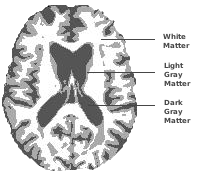
\includegraphics[width=2.2in]{Features.png}
\DeclareGraphicsExtensions.
\caption{Extracted Features}
\end{figure}
\subsection{ANN Implementation}
A neural network is modeled with a three neuron input layer, each corresponding to one of the extracted features. This model consists of two hidden layers and an output layer with two neurons each. The hidden layers use hyperbolic tangent function as activation function, mathematically expressed as:
\begin{equation}
f(x) = tanh(x) = \frac{2}{1+e^{-2x}} - 1 
\end{equation}
The model uses back propagation method for training.
\begin{figure}[h]
\centering
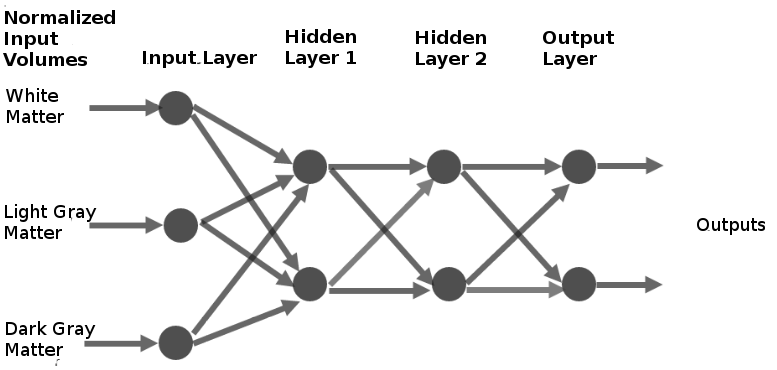
\includegraphics[scale=.3]{ANN.png}
\DeclareGraphicsExtensions.
\caption{ANN Model}
\end{figure}
\subsection{KNN Implementation}
A KNN model is designed where the 5-fold cross validation technique resulted in 7 as the best value of K (value of K for minimum classification error). So, the majority class of the 7 nearest neighbors of each input scan is assigned as the class for that scan. 
\par Nearest neighbor approximation is done by the measure of Eucledian Distance as given by:
\begin{equation}
\delta = \sqrt{ (G_{ip}-G_{tr})^2 +(g_{ip}-g_{tr})^2 +(W_{ip}-W_{tr})^2}
\end{equation}
Where,
\newline $\delta$ = Eucledian Distance
\newline $W_{ip}$ = Normalized volume of white matter of input image
\newline $g_{ip}$ = Normalized volume of light gray matter of input image
\newline $G_{ip}$ = Normalized volume of dark gray matter of input image
\newline $W_{tr}$ = Normalized volume of white matter of training image
\newline $g_{tr}$ = Normalized volume of light gray matter of training image
\newline $G_{tr}$ = Normalized volume of dark gray matter of training image
\section{Results}
\subsection{ANN Model Validation}
\noindent The following confusion matrix shows performance of the ANN model: \newline
\begin{table}[h!]
	\centering
	\begin{tabular}{|c|c|}
  		\hline
  		& \emph{Actual} \\
  		\hline
  		\emph{Predicted} & 
  		\begin{tabular}{c |c c c}
    	& Positive & Negative & Total \\
     	\hline
    	Positive & 18 & 9 & 27 \\
      	Negative & 7 & 19 & 26 \\
      	Total & 25 & 28 &  \\
		\end{tabular}
 		\\
  	\hline
	\end{tabular}
	\caption{Result from ANN Implementation}
\end{table}
\newline Accuracy : 69.81 \% 
\newline Sensitivity : 72.00\%
\newline Specificity : 67.85\%
\begin{figure}[h!]
\centering
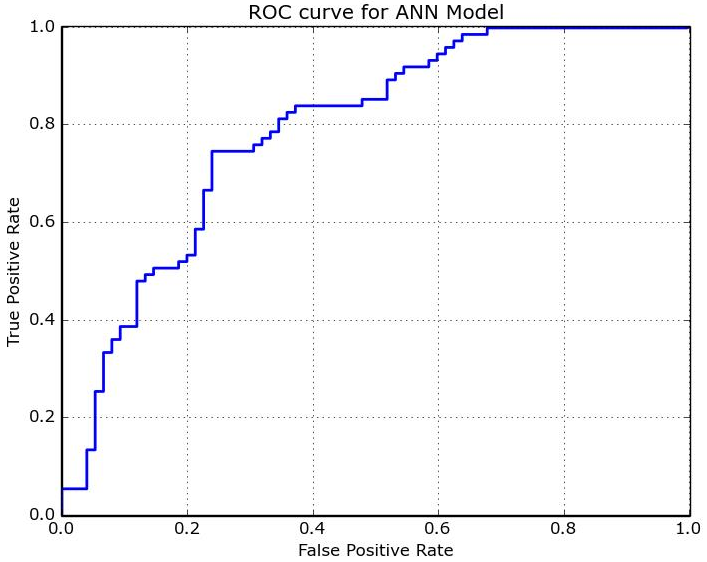
\includegraphics[scale=.32]{ANN_ROC.png}
\DeclareGraphicsExtensions.
\caption{ROC Curve for ANN Model}
\end{figure}
\newline
\par Out of the 53 test data, the ANN model resulted in 18 true positives and 19 true negatives along with 9 false positives and 7 false negatives. This means that the ANN model is able to identify positive dementia with a Positive Prediction Value (PPV) of 0.6666 and negative dementia with a Negative Prediction Value (NPV) of 0.7307.
\subsection{KNN Model Validation}
\par The following confusion matrix shows performance of the KNN model.
\newline
\begin{table}[h!]
	\centering
    \begin{tabular}{|c|c|}
  	\hline
  	& \emph{Actual} \\
  	\hline
  	\emph{Predicted} & 
  	\begin{tabular}{c |c c c}
    	& Positive & Negative & Total \\
        \hline
        Positive & 19 & 4 & 23 \\
        Negative & 6 & 24 & 30 \\
        Total & 25 & 28 &  \\
	\end{tabular}
 	\\
  	\hline
	\end{tabular}
    \caption{Results from KNN Implementation}
\end{table}
\newline Accuracy : 81.13\%
\newline Sensitivity : 76.00\%
\newline Specificity : 85.71\%
\begin{figure}[h!]
\centering
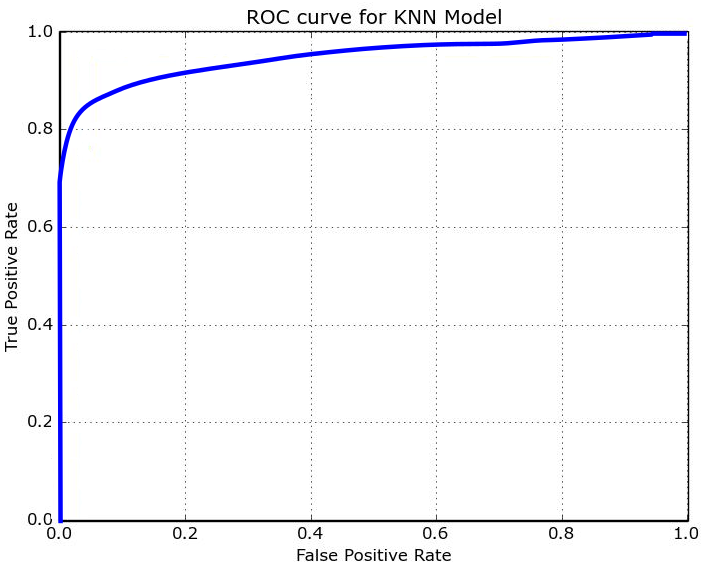
\includegraphics[scale=.40]{KNN_ROC.png}
\DeclareGraphicsExtensions.
\caption{ROC Curve for KNN Model}
\end{figure}
\newline
\par Out of the 53 test data, the KNN model resulted in 19 true positives and 24 true negatives along with 4 false positives and 6 false negative. This means that the KNN model is able to identify positive dementia with a Positive Prediction Value (PPV) of 0.8260 and negative dementia with a Negative Prediction Value (NPV) of 0.80.
\section{Conclusion}
From the above result, we can see that the KNN model has performed better than ANN model in all statistical measures of performance of binary classification models.
\par The KNN model produces adequate accuracy to be termed as a medically acceptable level of diagnosis accuracy($>$80\%) for the dataset used. This level of accuracy as given by the KNN model is better in comparison to many existing systems and within comparable bounds of several others.
\par Machine learning and artificial intelligence can produce significant accuracy in classification of demented and non-demented MRI scans. Further, artificial intelligence, if researched extensively, may some day surpass human accuracies in disease diagnosis and replace human expertise in the same.

\section{Future Work}
The OASIS repository provides limited datasets that can be used in KNN implementation and in training the ANN model. A larger dataset covering a wide range of subjects could improve the accuracies of these models and in verification of the results obtained. 
\par Further experimentation on the ANN could result into a better model for implementation in dementia diagnosis.
\par Further, the use of filters like median filter and fuzzy filter could reduce noise in the image leading to better accuracy.
% needed in second column of first page if using \IEEEpubid
%\IEEEpubidadjcol

% An example of a floating figure using the graphicx package.
% Note that \label must occur AFTER (or within) \caption.
% For figures, \caption should occur after the \includegraphics.
% Note that IEEEtran v1.7 and later has special internal code that
% is designed to preserve the operation of \label within \caption
% even when the captionsoff option is in effect. However, because
% of issues like this, it may be the safest practice to put all your
% \label just after \caption rather than within \caption{}.
%
% Reminder: the "draftcls" or "draftclsnofoot", not "draft", class
% option should be used if it is desired that the figures are to be
% displayed while in draft mode.
%
%\begin{figure}[!t]
%\centering
%\includegraphics[width=2.5in]{myfigure}
% where an .eps filename suffix will be assumed under latex, 
% and a .pdf suffix will be assumed for pdflatex; or what has been declared
% via \DeclareGraphicsExtensions.
%\caption{Simulation Results}
%\label{fig_sim}
%\end{figure}

% Note that IEEE typically puts floats only at the top, even when this
% results in a large percentage of a column being occupied by floats.


% An example of a double column floating figure using two subfigures.
% (The subfig.sty package must be loaded for this to work.)
% The subfigure \label commands are set within each subfloat command, the
% \label for the overall figure must come after \caption.
% \hfil must be used as a separator to get equal spacing.
% The subfigure.sty package works much the same way, except \subfigure is
% used instead of \subfloat.
%
%\begin{figure*}[!t]
%\centerline{\subfloat[Case I]\includegraphics[width=2.5in]{subfigcase1}%
%\label{fig_first_case}}
%\hfil
%\subfloat[Case II]{\includegraphics[width=2.5in]{subfigcase2}%
%\label{fig_second_case}}}
%\caption{Simulation results}
%\label{fig_sim}
%\end{figure*}
%
% Note that often IEEE papers with subfigures do not employ subfigure
% captions (using the optional argument to \subfloat), but instead will
% reference/describe all of them (a), (b), etc., within the main caption.


% An example of a floating table. Note that, for IEEE style tables, the 
% \caption command should come BEFORE the table. Table text will default to
% \footnotesize as IEEE normally uses this smaller font for tables.
% The \label must come after \caption as always.
%
%\begin{table}[!t]
%% increase table row spacing, adjust to taste
%\renewcommand{\arraystretch}{1.3}
% if using array.sty, it might be a good idea to tweak the value of
% \extrarowheight as needed to properly center the text within the cells
%\caption{An Example of a Table}
%\label{table_example}
%\centering
%% Some packages, such as MDW tools, offer better commands for making tables
%% than the plain LaTeX2e tabular which is used here.
%\begin{tabular}{|c||c|}
%\hline
%One & Two\\
%\hline
%Three & Four\\
%\hline
%\end{tabular}
%\end{table}


% Note that IEEE does not put floats in the very first column - or typically
% anywhere on the first page for that matter. Also, in-text middle ("here")
% positioning is not used. Most IEEE journals use top floats exclusively.
% Note that, LaTeX2e, unlike IEEE journals, places footnotes above bottom
% floats. This can be corrected via the \fnbelowfloat command of the
% stfloats package.




% if have a single appendix:
%\appendix[Proof of the Zonklar Equations]
% or
%\appendix  % for no appendix heading
% do not use \section anymore after \appendix, only \section*
% is possibly needed

% use appendices with more than one appendix
% then use \section to start each appendix
% you must declare a \section before using any
% \subsection or using \label (\appendices by itself
% starts a section numbered zero.)

%\appendices
%\section{Something Goes Here, but what?}
%Some text for the appendix.

% use section* for acknowledgement
\section*{Acknowledgment}
The authors would like to acknowledge the support of the OASIS project by grants P50 AG05681, P01 AG03991, R01 AG021910, P50 MH071616, U24 RR021382 and R01 MH56584.
\par The authors would also like to acknowledge the support the Department of Electronics and Computer Engineering at Central Campus, Institute of Engineering, Tribhuvan University.



% Can use something like this to put references on a page
% by themselves when using endfloat and the captionsoff option.
\ifCLASSOPTIONcaptionsoff
  \newpage
\fi



% trigger a \newpage just before the given reference
% number - used to balance the columns on the last page
% adjust value as needed - may need to be readjusted if
% the document is modified later
%\IEEEtriggeratref{8}
% The "triggered" command can be changed if desired:
%\IEEEtriggercmd{\enlargethispage{-5in}}

% references section

% can use a bibliography generated by BibTeX as a .bbl file
% BibTeX documentation can be easily obtained at:
% http://www.ctan.org/tex-archive/biblio/bibtex/contrib/doc/
% The IEEEtran BibTeX style support page is at:
% http://www.michaelshell.org/tex/ieeetran/bibtex/
%\bibliographystyle{IEEEtran}
% argument is your BibTeX string definitions and bibliography database(s)
%\bibliography{IEEEabrv,../bib/paper}
%
% <OR> manually copy in the resultant .bbl file
% set second argument of \begin to the number of references
% (used to reserve space for the reference number labels box)
\begin{thebibliography}{1}
%\bibitem{IEEEhowto:kopka}
%H.~Kopka and P.~W. Daly, \emph{A Guide to \LaTeX}, 3rd~ed. Harlow, England: Addison-Wesley, 1999.
\bibitem{}
Alzheimer's Association, \emph{2015 Alzheimer\textquotesingle s Disease Facts and Figures}. Alzheimer's \& Dementia 2015.
\bibitem{}
Alzhiemer\textquotesingle s Australia, \emph{Dementia Q\&A: Tests Used in Diagnosing Dementia}, 2014.     
\bibitem{}
J.~Valk, F.~Barkhof and P.~Scheltens, \emph{Magnetic Resonance in Dementia}: Springer-Verlag Berlin Heidelberg, New York, 2002.
\bibitem{}
W.~R. Shankleab, S.~Mania, M.~B. Dickc and M.~J. Pazzania, \emph{Simple Models for Estimating Dementia Severity Using Machine Learning}, Studies in Health Technology and Informatics: University of California at Irvine, Irvine, California, 1998.
\bibitem{}
V.~Miller, S.~Erlien, and J.~Piersol, \emph{Identifying dementia in MRI scans using machine learning}, Stanford University, Stanford, CA.
\bibitem{}
W.~R. Shankle, P.~Datta, M.~Dillencourt and M.~Pazzani, \emph{Improving Dementia Screening Tests with Machine Learning Methods}, Alzheimer’s Research: University of California at Irvine, Irvine, CA, 1996.
\bibitem{}
J.~A. Williams, A.~Weakley, D.~J. Cook and M~.Schmitter-Edgecombe, \emph{Machine Learning Techniques for Diagnostic Differentiation of Mild Cognitive Impairment and Dementia}, AAAI  2013  Workshop, Expanding  the Boundaries of Health Informatics using Artificial Intelligence, Washington State University, Pullman, WA.
\bibitem{}
P.~Datta, W.~R. Shankle and M.~Pazzani, \emph{Applying Machine Learning to an Alzheimer's Database}, AAAI-96 Spring Symposium, AI in Medicine: Applications of Current Technologies: University of California at Irvine, Irvine, CA, 1996.
\bibitem{}
K.~R. Gray, \emph{Machine learning for image-based classification of Alzheimer’s disease}, Imperial College London, UK.
\bibitem{}
D. S. Marcus, T. H. Wang, J. Parker, J. G. Csernansky, J. C. Morris, and R. L. Buckner, \emph{OASIS Fact Sheet: Cros-Sectional Data Across The Adult Lifespan}, Journal of Cognitive Neuroscience, 2007.
\bibitem{}
M.~Sezgin and B.~Sankur, \emph{Survey over image thresholding techniques and quantitative performance evaluation}, Journal of Electronic Imaging 13(1), 146–165,January 2004.
\bibitem{}
L.~M. Surhone, M.~T. Timpledon and S.~F. Marseken, \emph{Nearest - Neighbor Interpolation}, VDM Publishing, 2010.
\bibitem{}
M.~Hassoun, \emph{Fundamentals of Artificial Neural Networks}: The MIT Press, Cambridge, Massachusetts, 1995.
\bibitem{} 
E.~Deza, M.~M. Deza, \emph{Encyclopedia of Distances}: Springer-Verlag, Berlin, Heidelberg. 2009.
\bibitem{}
Gerardnico, \emph{Machine Learning - K-Nearest Neighbors (KNN) algorithm - Instance based learning}    
\end{thebibliography}

\begin{IEEEbiography}[{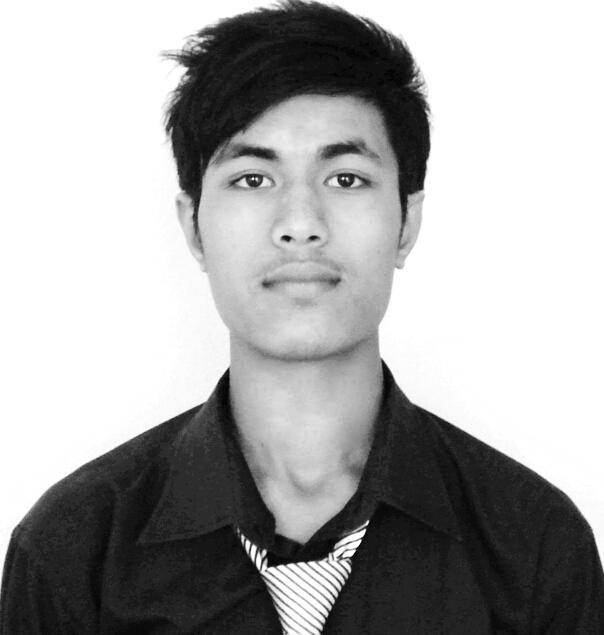
\includegraphics[width=1in,height=1.25in,clip,keepaspectratio]{author1.jpg}}]{Abinash Manandhar} studied Bachelors in Computer Engineering at Pulchowk Campus, Tribhuvan University, Institute of Engineering. He is a data science enthusiast and is currently a trainee at the Kathmandu offices of EB Pearls Australia Pty. Ltd.
\end{IEEEbiography}
\vspace{-1cm}
\begin{IEEEbiography}[{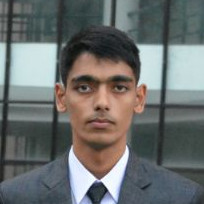
\includegraphics[width=1in,height=1.15in,clip,keepaspectratio]{author2.jpg}}]{Sagar Gautam} was born in Gulmi, Western Nepal. He received his Bachelors degree in Computer Engineering from Tribhuvan University, Institute of Engineering. His interests are in the fields of machine learning and artificial intelligence.
\end{IEEEbiography}
\vspace{-1cm}
\begin{IEEEbiography}[{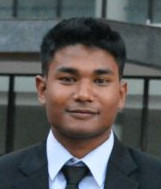
\includegraphics[width=1in,height=1.15in,clip,keepaspectratio]{author3.jpg}}]{Dharma Krishna Shrestha} studied Bachelors in Computer Engineering at Tribhuvan University, Institute of Engineering. Born in Bhaktapur, he has his interests in biometry and image processing.
\end{IEEEbiography}
\vspace{-1cm}
\begin{IEEEbiography}[{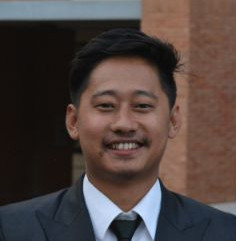
\includegraphics[width=1in,height=1.15in,clip,keepaspectratio]{author4.jpg}}]{Sujan Sauden} was born in Pathari, Eastern Nepal. He studied Bachelors in Computer Engineering at Tribhuvan University, Institute of Engineering. He currently works at Kul Techno Lab and Research Centre, Kathmandu.
\end{IEEEbiography}
\vspace{-1cm}
\begin{IEEEbiography}[{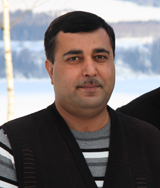
\includegraphics[width=1in,height=1.25in,clip,keepaspectratio]{author5.jpg}}]{Dibakar Raj pant} is the Department Head of the Department of Electronics \& Computer Engineering at Pulchowk Campus, Tribhuvan University, Institute of Engineering. He received his MSc degree from the University of Joensuu, Finland, his PhD in Images, Vision and Signal from the Jean Monnet University, France and his post doctoral degree from Gj\o vik University College, Oppland County, Norway. He has his background in Color and Imaging, Machine learning and Pattern Recognition, Statistical Data Analysis and Electrical \and Electronics Engineering. 
\end{IEEEbiography}
%\section*{Correspondence Information}
%Correspondence concerning this article should be addressed to Abinash Manandhar, Department of Electronics and Computer Engineering, Central Campus, Institute of Engineering, Tribhuvan University.
%\newline Contact: abinash.mdr@gmail.com

% biography section
% 
% If you have an EPS/PDF photo (graphicx package needed) extra braces are
% needed around the contents of the optional argument to biography to prevent
% the LaTeX parser from getting confused when it sees the complicated
% \includegraphics command within an optional argument. (You could create
% your own custom macro containing the \includegraphics command to make things
% simpler here.)
%\begin{biography}[{\includegraphics[width=1in,height=1.25in,clip,keepaspectratio]{mshell}}]{Michael Shell}
% or if you just want to reserve a space for a photo:

%\begin{IEEEbiography}[{\includegraphics[width=1in,height=1.25in,clip,keepaspectratio]{picture}}]{John Doe}
%\end{IEEEbiography}

% You can push biographies down or up by placing
% a \vfill before or after them. The appropriate
% use of \vfill depends on what kind of text is
% on the last page and whether or not the columns
% are being equalized.

%\vfill

% Can be used to pull up biographies so that the bottom of the last one
% is flush with the other column.
%\enlargethispage{-5in}




% that's all folks
\end{document}


